% Practice Test 14 — Alaska Edition
% Questions: 30 (21 MC + 9 SA)
% Generated by scripts/generate_practice_tests.py

\begin{practiceQuestion}{1-3-q02}{mc}
\begin{questionText}
In a proportional relationship, the constant of proportionality $k$ equals:
\end{questionText}
\choiceA{$x \div y$}
\choiceB{$y \div x$}
\choiceC{$x \times y$}
\choiceD{$y - x$}
\correctAnswer{B}
\explanation{The constant of proportionality is $k = \frac{y}{x}$, which is the unit rate.}
\end{practiceQuestion}

\begin{practiceQuestion}{1-5-q22}{sa}
\begin{questionText}
Explain what the point $(0, 0)$ means on a graph of cost versus number of books purchased.
\end{questionText}
\correctAnswer{Buying $0$ books costs $\$0$}
\explanation{The origin means both quantities are zero: zero books and zero cost. This confirms no fixed fee.}
\end{practiceQuestion}

\begin{practiceQuestion}{1-6-q08}{mc}
\begin{questionText}
A machine fills $350$ bottles in $5$ hours. How many bottles does it fill in $12$ hours?
\end{questionText}
\choiceA{$700$}
\choiceB{$780$}
\choiceC{$840$}
\choiceD{$900$}
\correctAnswer{C}
\explanation{Rate: $350 \div 5 = 70$ bottles/hr. In $12$ hours: $70 \times 12 = 840$ bottles.}
\end{practiceQuestion}

\begin{practiceQuestion}{2-2-q29}{gsa}
\begin{questionText}
The double number line below shows a percent relationship. What number goes at the question mark?

\begin{center}
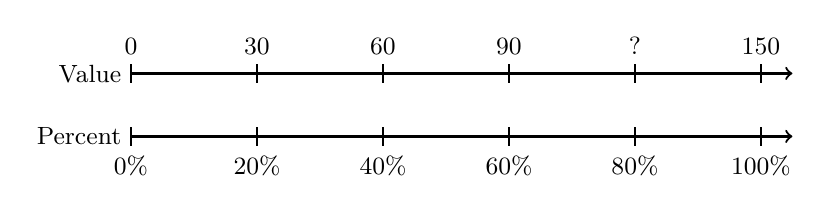
\begin{tikzpicture}[scale=0.8]
  % Top number line (values)
  \draw[thick,->] (0,1) -- (10.5,1);
  \node[left,font=\small] at (0,1) {Value};
  \foreach \x/\lab in {0/0, 2/30, 4/60, 6/90, 8/?, 10/150} {
    \draw[thick] (\x,0.85) -- (\x,1.15);
    \node[above,font=\small] at (\x,1.15) {\lab};
  }
  % Bottom number line (percent)
  \draw[thick,->] (0,0) -- (10.5,0);
  \node[left,font=\small] at (0,0) {Percent};
  \foreach \x/\lab in {0/0\%, 2/20\%, 4/40\%, 6/60\%, 8/80\%, 10/100\%} {
    \draw[thick] (\x,-0.15) -- (\x,0.15);
    \node[below,font=\small] at (\x,-0.15) {\lab};
  }
\end{tikzpicture}
\end{center}
\end{questionText}
\correctAnswer{$120$}
\explanation{The whole ($100\%$) corresponds to $150$. At $80\%$: $\frac{n}{150} = \frac{80}{100}$ → $n = 120$.}
\end{practiceQuestion}

\begin{practiceQuestion}{2-5-q29}{gsa}
\begin{questionText}
The receipt below shows a restaurant bill. Calculate the $18\%$ tip and the total amount.

\begin{center}
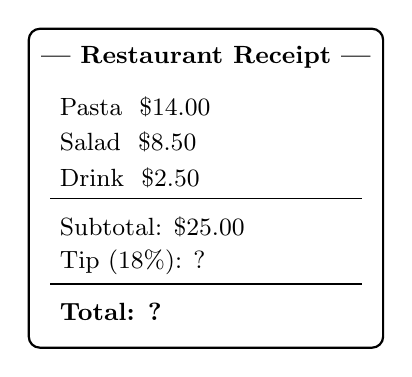
\begin{tikzpicture}[scale=0.9]
  \draw[thick,rounded corners] (0,0) rectangle (5,4.5);
  \node[font=\small\bfseries] at (2.5,4.1) {--- Restaurant Receipt ---};
  \node[anchor=west,font=\small] at (0.3,3.4) {Pasta \dotfill\ $\$14.00$};
  \node[anchor=west,font=\small] at (0.3,2.9) {Salad \dotfill\ $\$8.50$};
  \node[anchor=west,font=\small] at (0.3,2.4) {Drink \dotfill\ $\$2.50$};
  \draw[thin] (0.3,2.1) -- (4.7,2.1);
  \node[anchor=west,font=\small] at (0.3,1.7) {Subtotal: $\$25.00$};
  \node[anchor=west,font=\small] at (0.3,1.2) {Tip (18\%): ?};
  \draw[thick] (0.3,0.9) -- (4.7,0.9);
  \node[anchor=west,font=\small\bfseries] at (0.3,0.5) {Total: ?};
\end{tikzpicture}
\end{center}
\end{questionText}
\correctAnswer{Tip $= \$4.50$; Total $= \$29.50$}
\explanation{Tip: $25.00 \times 0.18 = \$4.50$. Total: $25.00 + 4.50 = \$29.50$.}
\end{practiceQuestion}

\begin{practiceQuestion}{3-1-q20}{sa}
\begin{questionText}
Find $|{-23}|$.
\end{questionText}
\correctAnswer{$23$}
\explanation{The absolute value of $-23$ is its distance from $0$, which is $23$.}
\end{practiceQuestion}

\begin{practiceQuestion}{3-2-q22}{sa}
\begin{questionText}
What is $(-18) + 18$?
\end{questionText}
\correctAnswer{$0$}
\explanation{$-18$ and $18$ are additive inverses (opposites). Their sum is always $0$.}
\end{practiceQuestion}

\begin{practiceQuestion}{3-3-q24}{sa}
\begin{questionText}
Evaluate: $15 - 22 - (-4)$.
\end{questionText}
\correctAnswer{$-3$}
\explanation{$15 - 22 = 15 + (-22) = -7$. Then $-7 - (-4) = -7 + 4 = -3$.}
\end{practiceQuestion}

\begin{practiceQuestion}{3-10-q18}{mc}
\begin{questionText}
Evaluate: $(-2.4) \times 5 - (-3.8)$
\end{questionText}
\choiceA{$-15.8$}
\choiceB{$-8.2$}
\choiceC{$8.2$}
\choiceD{$15.8$}
\correctAnswer{B}
\explanation{$(-2.4) \times 5 = -12$. Then $-12 - (-3.8) = -12 + 3.8 = -8.2$.}
\end{practiceQuestion}

\begin{practiceQuestion}{4-1-q17}{mc}
\begin{questionText}
An amusement park charges an entrance fee of $\$25$ and $\$4$ per ride. Maria has $\$53$. Which expression shows how much money she has left after going on $r$ rides?
\end{questionText}
\choiceA{$53 - 25 - 4r$}
\choiceB{$53 - 29r$}
\choiceC{$53 - 4r$}
\choiceD{$25 + 4r - 53$}
\correctAnswer{A}
\explanation{She pays $\$25$ entrance and $\$4$ per ride ($4r$). Remaining: $53 - 25 - 4r$.}
\end{practiceQuestion}

\begin{practiceQuestion}{5-2-q07}{mc}
\begin{questionText}
Solve $\dfrac{n}{6} - 5 = 3$.
\end{questionText}
\choiceA{$n = 48$}
\choiceB{$n = -12$}
\choiceC{$n = 18$}
\choiceD{$n = 12$}
\correctAnswer{A}
\explanation{Add $5$: $\frac{n}{6} = 8$. Multiply by $6$: $n = 48$. Check: $\frac{48}{6} - 5 = 8 - 5 = 3$ \checkmark.}
\end{practiceQuestion}

\begin{practiceQuestion}{5-3-q06}{mc}
\begin{questionText}
Which equation is equivalent to $4(x + 5) = 36$?
\end{questionText}
\choiceA{$4x + 5 = 36$}
\choiceB{$4x + 20 = 36$}
\choiceC{$4x + 9 = 36$}
\choiceD{$x + 20 = 36$}
\correctAnswer{B}
\explanation{Distribute $4$: $4 \times x + 4 \times 5 = 4x + 20$. So the equation becomes $4x + 20 = 36$.}
\end{practiceQuestion}

\begin{practiceQuestion}{5-4-q28}{gmc}
\begin{questionText}
The thermometer shows the current temperature. The temperature was $-3.5\degree$F this morning and rose $t$ degrees each hour for $4$ hours to reach the current reading. What is $t$?

\begin{center}
\begin{tikzpicture}[scale=0.5]
  % Thermometer
  \draw[thick] (0,0) -- (0,10) arc(180:0:0.5) -- (1,0) arc(0:-180:0.5);
  \fill[red!60] (0.1,0) rectangle (0.9,6.5);
  % Scale
  \foreach \y/\val in {0/-5, 2/0, 4/5, 6/10, 8/15, 10/20} {
    \draw (-0.3,\y) -- (0,\y);
    \node[left] at (-0.4,\y) {$\val\degree$F};
  }
  % Arrow to current
  \draw[thick,->,funBlue] (1.8,6.5) -- (1.1,6.5);
  \node[right] at (1.8,6.5) {Current: $8.5\degree$F};
\end{tikzpicture}
\end{center}
\end{questionText}
\choiceA{$t = 3$}
\choiceB{$t = 5$}
\choiceC{$t = 1.25$}
\choiceD{$t = 2$}
\correctAnswer{A}
\explanation{Equation: $-3.5 + 4t = 8.5$. Add $3.5$: $4t = 12$. Divide by $4$: $t = 3$.}
\end{practiceQuestion}

\begin{practiceQuestion}{5-5-q04}{mc}
\begin{questionText}
Solve $5x - 10 \geq 25$.
\end{questionText}
\choiceA{$x \geq 3$}
\choiceB{$x \geq 7$}
\choiceC{$x \leq 7$}
\choiceD{$x \geq 35$}
\correctAnswer{B}
\explanation{Add $10$: $5x \geq 35$. Divide by $5$: $x \geq 7$.}
\end{practiceQuestion}

\begin{practiceQuestion}{5-6-q01}{mc}
\begin{questionText}
What type of circle is used to graph $x > 3$ on a number line?
\end{questionText}
\choiceA{Closed circle at $3$}
\choiceB{Open circle at $3$}
\choiceC{Closed circle at $0$}
\choiceD{Open circle at $0$}
\correctAnswer{B}
\explanation{$x > 3$ uses an open circle because $3$ is not included (strictly greater than).}
\end{practiceQuestion}

\begin{practiceQuestion}{6-2-q03}{mc}
\begin{questionText}
A model uses scale $1:100$. You need to redraw it at scale $1:50$. A wall that is $4$ cm on the original model becomes how long?
\end{questionText}
\choiceA{$2$ cm}
\choiceB{$4$ cm}
\choiceC{$8$ cm}
\choiceD{$200$ cm}
\correctAnswer{C}
\explanation{Scale ratio: $\frac{100}{50} = 2$. New length: $4 \times 2 = 8$ cm.}
\end{practiceQuestion}

\begin{practiceQuestion}{6-3-q17}{mc}
\begin{questionText}
A triangle has side lengths $9$, $12$, and $15$. What type of triangle is it?
\end{questionText}
\choiceA{Equilateral}
\choiceB{Isosceles}
\choiceC{Right}
\choiceD{It cannot be formed}
\correctAnswer{C}
\explanation{Check: $9^2 + 12^2 = 81 + 144 = 225 = 15^2$. Since the Pythagorean theorem holds, this is a right triangle.}
\end{practiceQuestion}

\begin{practiceQuestion}{6-4-q26}{gmc}
\begin{questionText}
The diagram shows a triangle with the given angle measures. Is this a valid triangle?

\begin{center}
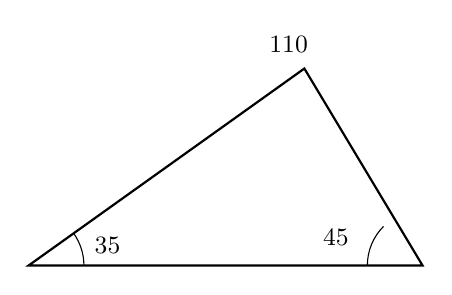
\begin{tikzpicture}[scale=1]
  \draw[thick] (0,0) -- (5,0) -- (3.5,2.5) -- cycle;
  \draw (0.7,0) arc[start angle=0,end angle=35,radius=0.7];
  \node at (1.0,0.25) {\small $35°$};
  \draw (4.3,0) arc[start angle=180,end angle=135,radius=0.7];
  \node at (3.9,0.35) {\small $45°$};
  \node at (3.3,2.8) {\small $110°$};
\end{tikzpicture}
\end{center}
\end{questionText}
\choiceA{Yes, because $35 + 45 + 110 = 190$}
\choiceB{Yes, because all angles are positive}
\choiceC{No, because the angles sum to $190°$ instead of $180°$}
\choiceD{No, because one angle is greater than $90°$}
\correctAnswer{C}
\explanation{$35 + 45 + 110 = 190 \neq 180$. Triangle angles must sum to exactly $180°$, so this triangle is not valid.}
\end{practiceQuestion}

\begin{practiceQuestion}{6-5-q12}{mc}
\begin{questionText}
A rectangular prism is sliced with a diagonal cut from one edge of the top to the opposite edge of the bottom. What is a possible cross-section?
\end{questionText}
\choiceA{Circle}
\choiceB{Triangle}
\choiceC{Hexagon}
\choiceD{Rectangle}
\correctAnswer{D}
\explanation{A diagonal slice through a rectangular prism from edge to edge can produce a rectangle (or a parallelogram, depending on the angle). A diagonal from top edge to opposite bottom edge typically gives a rectangle.}
\end{practiceQuestion}

\begin{practiceQuestion}{7-3-q20}{sa}
\begin{questionText}
A circular garden has a diameter of $20$ meters. What is its area? Use $\pi \approx 3.14$.
\end{questionText}
\correctAnswer{$314$ m$^2$}
\explanation{$r = 10$ m. $A = \pi r^2 = 3.14 \times 100 = 314$ m$^2$.}
\end{practiceQuestion}

\begin{practiceQuestion}{7-4-q06}{mc}
\begin{questionText}
An L-shaped room can be split into a $10$ ft by $8$ ft rectangle and a $4$ ft by $6$ ft rectangle. What is the total floor area?
\end{questionText}
\choiceA{$56$ ft$^2$}
\choiceB{$80$ ft$^2$}
\choiceC{$104$ ft$^2$}
\choiceD{$128$ ft$^2$}
\correctAnswer{C}
\explanation{$10 \times 8 = 80$ ft$^2$. $4 \times 6 = 24$ ft$^2$. Total: $80 + 24 = 104$ ft$^2$.}
\end{practiceQuestion}

\begin{practiceQuestion}{7-5-q22}{sa}
\begin{questionText}
A cube has a surface area of $384$ in$^2$. What is the side length?
\end{questionText}
\correctAnswer{$8$ in}
\explanation{$s^2 = 384 \div 6 = 64$. So $s = 8$ in.}
\end{practiceQuestion}

\begin{practiceQuestion}{7-6-q28}{gmc}
\begin{questionText}
A triangular prism is shown below. What is its volume?

\begin{center}
\begin{tikzpicture}[scale=0.35]
  % Front triangle
  \fill[funBlue!10] (0,0) -- (8,0) -- (4,5) -- cycle;
  \draw[thick,funBlue] (0,0) -- (8,0) -- (4,5) -- cycle;
  % Back triangle
  \fill[funBlue!20] (3,2) -- (11,2) -- (7,7) -- cycle;
  \draw[thick,funBlue] (3,2) -- (11,2) -- (7,7) -- cycle;
  % Connecting edges
  \draw[thick,funBlue] (0,0) -- (3,2);
  \draw[thick,funBlue] (8,0) -- (11,2);
  \draw[thick,funBlue] (4,5) -- (7,7);
  % Labels
  \draw[thick,funRed,<->] (0,-0.8) -- (8,-0.8);
  \node[below,funRed] at (4,-0.8) {$8$ m};
  \draw[dashed,gray] (4,0) -- (4,5);
  \node[left,funRed] at (3.8,2.5) {$5$ m};
  \node[right,funRed] at (11.2,4.5) {$12$ m};
\end{tikzpicture}
\end{center}
\end{questionText}
\choiceA{$120$ m$^3$}
\choiceB{$240$ m$^3$}
\choiceC{$480$ m$^3$}
\choiceD{$96$ m$^3$}
\correctAnswer{B}
\explanation{$B = \frac{1}{2} \times 8 \times 5 = 20$ m$^2$. $V = 20 \times 12 = 240$ m$^3$.}
\end{practiceQuestion}

\begin{practiceQuestion}{8-1-q06}{mc}
\begin{questionText}
A city wants to survey residents about a new park. Which method would produce the least biased sample?
\end{questionText}
\choiceA{Survey people at the existing park}
\choiceB{Put the survey in the newspaper and wait for responses}
\choiceC{Randomly select addresses from the city directory}
\choiceD{Survey people at the city council meeting}
\correctAnswer{C}
\explanation{Randomly selecting addresses gives all residents an equal chance, reducing bias.}
\end{practiceQuestion}

\begin{practiceQuestion}{8-3-q25}{sa}
\begin{questionText}
Two groups have means of $50$ and $54$, and both have MAD $= 8$. Express the difference in means as a multiple of MAD. Is the difference meaningful?
\end{questionText}
\correctAnswer{$0.5$ MADs; no, the difference is not meaningful}
\explanation{$\frac{54-50}{8} = 0.5$ MADs. Since $0.5 < 2$, the difference is small relative to the variability and not considered meaningful.}
\end{practiceQuestion}

\begin{practiceQuestion}{8-4-q27}{gmc}
\begin{questionText}
The box plots show quiz scores (out of $20$) for two classes.

\begin{center}
\begin{tikzpicture}[scale=0.35]
  \draw[thick,->] (4,0) -- (21,0);
  \foreach \x in {5,6,...,20} {
    \draw (\x,0.3) -- (\x,-0.3);
    \node[below,font=\tiny] at (\x,-0.3) {$\x$};
  }
  % Class M: min=8, Q1=12, med=15, Q3=17, max=20
  \draw[thick] (8,3) -- (20,3);
  \draw[thick,fill=funBlue!30] (12,2) rectangle (17,4);
  \draw[very thick,funBlue] (15,2) -- (15,4);
  \draw[thick] (8,2) -- (8,4);
  \draw[thick] (20,2) -- (20,4);
  \node[right,font=\small] at (20.5,3) {Class M};
  % Class N: min=10, Q1=13, med=16, Q3=18, max=19
  \draw[thick] (10,7) -- (19,7);
  \draw[thick,fill=funGreen!30] (13,6) rectangle (18,8);
  \draw[very thick,funGreen] (16,6) -- (16,8);
  \draw[thick] (10,6) -- (10,8);
  \draw[thick] (19,6) -- (19,8);
  \node[right,font=\small] at (19.5,7) {Class N};
\end{tikzpicture}
\end{center}

What is the IQR for each class?
\end{questionText}
\choiceA{Class M: $5$, Class N: $5$}
\choiceB{Class M: $12$, Class N: $9$}
\choiceC{Class M: $5$, Class N: $9$}
\choiceD{Class M: $12$, Class N: $5$}
\correctAnswer{A}
\explanation{Class M: $Q_3 - Q_1 = 17 - 12 = 5$. Class N: $18 - 13 = 5$. Both have IQR $= 5$.}
\end{practiceQuestion}

\begin{practiceQuestion}{8-7-q09}{mc}
\begin{questionText}
Which display is best for comparing exact frequencies of categorical data?
\end{questionText}
\choiceA{Line graph}
\choiceB{Frequency table}
\choiceC{Box plot}
\choiceD{Dot plot}
\correctAnswer{B}
\explanation{A frequency table lists exact counts for each category, which is ideal for comparing categorical data.}
\end{practiceQuestion}

\begin{practiceQuestion}{9-4-q16}{mc}
\begin{questionText}
A game has $4$ outcomes: Win Big, Win Small, Lose Small, Lose Big. The probabilities are $0.05$, $0.25$, $0.45$, and $0.25$. Which outcome is LEAST likely?
\end{questionText}
\choiceA{Win Big}
\choiceB{Win Small}
\choiceC{Lose Small}
\choiceD{Lose Big}
\correctAnswer{A}
\explanation{Win Big has the smallest probability ($0.05$), making it least likely.}
\end{practiceQuestion}

\begin{practiceQuestion}{9-6-q11}{mc}
\begin{questionText}
Two dice are rolled. What is the probability that the sum is even?
\end{questionText}
\choiceA{$\frac{1}{4}$}
\choiceB{$\frac{1}{3}$}
\choiceC{$\frac{1}{2}$}
\choiceD{$\frac{2}{3}$}
\correctAnswer{C}
\explanation{Even sums occur when both dice are even or both are odd. Both even: $3 \times 3 = 9$. Both odd: $3 \times 3 = 9$. Total: $18$ out of $36$. $P = \frac{18}{36} = \frac{1}{2}$.}
\end{practiceQuestion}

\begin{practiceQuestion}{9-7-q03}{mc}
\begin{questionText}
To simulate an event with a $\frac{1}{6}$ probability, which tool would be most appropriate?
\end{questionText}
\choiceA{A coin}
\choiceB{A standard die}
\choiceC{A spinner with $4$ sections}
\choiceD{A bag with $2$ marbles}
\correctAnswer{B}
\explanation{A standard die has $6$ equally likely outcomes, each with probability $\frac{1}{6}$.}
\end{practiceQuestion}
